% \title{ Сравнение подходов обучения на базе словаря и MAP к проблеме повышения разрешения на примере изображений автомобильных номеров }
\title{Повышение разрешения изображений автомобильных номеров}
\author{
  \begin{tabular}[4cm]{rl}
 Автор:                & Улитин А.~А., 461 гр. \\
 Научный руководитель: & к.\,ф.-м.\,н., доцент~Вахитов А.~Т. \\
 Рецензент: & инженер-программист Пименов А. А. \\
 \end{tabular}
 }
\date{2013 год}

\begin{frame}{}
		\maketitle
\end{frame}

\section{Задача}
\begin{frame}{Задача Super-resolution}
  Задача Super resolution --- качественно повысить разрешения изображения.
  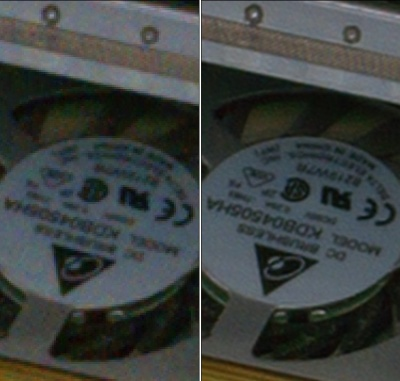
\includegraphics[height=\textheight]{content/An_example_of_super_resolution_with_still_RAW_photo.jpg}
\end{frame}

\begin{frame}{Почему это возможно}
  Для повышения разрешения используется дополнительная информация
  \begin{itemize}
    \item Знание параметров съемки (размытие, движение камеры~и~т.п.)
    \item Знание о типе снимаемого объекта (текст, лица, и т.п.)
    \item Использование нескольких изображений, снятых с разных ракурсов
  \end{itemize}
  которая влияет на конечное изображение

  Применимость:
  \begin{itemize}
    \item Препроцессинг для других алгоритмов компьютерного зрения
    \item Извлечение дополнительной информации с нескольких снимков для получения одного кадра с высоким разрешением
  \end{itemize}
\end{frame}

\begin{frame}{PSNR}

  $$ \mathrm{MSE}(\tilde{x},x) = \frac{1}{m\,n}\sum_{i=0}^{m-1}\sum_{j=0}^{n-1} [\tilde{x}(i,j) - x(i,j)]^2$$

  И обозначим величину обратную ей и выраженную на логарифмической шкале как $\mathrm{PSNR}(\tilde{x},x)$.
  $$ \mathrm{PSNR}(\tilde{x},x) &= 10 \cdot \log_{10} \left( \frac{\mathrm{MAX}_I^2}{\mathrm{MSE}(\tilde{x},x)} \right)
  $$
Где $MAX_I$ максимально возможное значение яркости изображения
\end{frame}

\begin{frame}{Постановка задачи}
 $$y_r = D H_R W_R x + n_r,~ ~ ~ 1 \leq r \leq m$$
 где:
 \begin{itemize}
   \item $x$ оригинальное изображение
   \item $y_r$ наблюдение r
   \item $D$ матрица понижение разрешения
   \item $W$ матрица геометрического искажения
   \item $H_R$ матрица размытия наблюдения r
   \item $n_r$ шум наблюдения r
   \item $m$ количество наблюдений
 \end{itemize}
 Задача найти
 $$ \tilde{x} = \underset{\hat{x}}{\operatorname{argmax}}~  PSNR(\hat{x},x)$$
\end{frame}
\section{Подходы}
\begin{frame}{Сравниваемые подходы}
  \begin{itemize}
    \item Couple Dictionary Training for Image Super-resolution \\
        (Jianchao Yang,Zhaowen Wang, Zhe Lin,Scott Cohen, and Thomas Huang) \\
  Основная идея метода очень проста -- тренировка словаря из патчей небольшого размера в двух разрешениях LR и HR
      \begin{itemize}
        \item Использует пару тренированных словарей
        \item Восстановление по одному изображению
      \end{itemize}
    \item Superresolution of License Plates in Real Traffic Videos \\
      (K. V. Suresh, G. Mahesh Kumar, and A. N. Rajagopalan) \\
      Основная идея -- использование шаговой оптимизации с адаптивным регуляризатором.
      \begin{itemize}
        \item Для восстановление использует последовательную оптимизацию с
          регуляризаторами
        \item Использует несколько изображений
      \end{itemize}
  \end{itemize}
\end{frame}

%\section{Описание подходов}
%\begin{frame}{Подход с тренированными словарями}
%\end{frame}

% \newcommand{\inimage}[2]{
%   \begin{minipage}{#1}
%     \vcenter{\includegraphics[width=\columnwidth]{#2}}
%   \end{minipage}
% }
%
%
% \section{Приведение изображений}
% \begin{frame}{Несколько изображение $\rightarrow$ одно изображение}
%   Для тестирования на однинаковых наборах данных из lr строились псевдо hr для
%   первого алгоритма методом:
%   $$ R = \frac{1}{n}\sum_{i=1}^nW^T \cdot S \cdot IMG_{lr i}$$
%   $S$ --- билинейная интерполяция \\
%   $W$ --- сдвиг
%
%   \inimage{3cm}{content/imgs/append_imgs_big.jpg}
%   $\to$
%   \inimage{6cm}{content/imgs/combined_big.jpg}
% \end{frame}

\begin{frame}{Исходные изображения}
  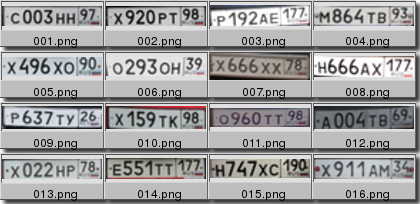
\includegraphics[width=\columnwidth]{content/out_sr1.png}
\end{frame}

\section{SR1}
\begin{frame}{Результаты подхода алгоритма со словарями}
  % This file was created by matlab2tikz v0.3.3.
% Copyright (c) 2008--2013, Nico Schlömer <nico.schloemer@gmail.com>
% All rights reserved.
% 
% The latest updates can be retrieved from
%   http://www.mathworks.com/matlabcentral/fileexchange/22022-matlab2tikz
% where you can also make suggestions and rate matlab2tikz.
% 
% 
% 
\begin{tikzpicture}

\begin{axis}[%
width=10cm,
height=7.88709677419355cm,
scale only axis,
xmin=0,
xmax=16,
xlabel={Номер изображения},
ymin=14,
ymax=28,
ylabel={PSNR dB},
legend style={draw=black,fill=white,legend cell align=left}
]
\addplot [
color=blue,
solid
]
table[row sep=crcr]{
1 22.6637207689603\\
2 16.5862621065916\\
3 20.2561814850212\\
4 16.8180326138836\\
5 15.2818944883097\\
6 20.8935173361133\\
7 19.9100975616132\\
8 21.8054095243458\\
9 19.5938529440994\\
10 14.97066690973\\
11 17.6444789637467\\
12 19.6591796988059\\
13 24.5276502442069\\
14 19.6886965973242\\
15 18.0639264824657\\
16 22.7687595823891\\
};
\addlegendentry{Алгоритм с обучаемыми словарями};

\addplot [
color=green!50!black,
dashed
]
table[row sep=crcr]{
1 20.654183811932\\
2 15.5287572495406\\
3 14.6873141103361\\
4 16.906444307724\\
5 16.6431061328363\\
6 15.8814467785726\\
7 15.7004358294634\\
8 20.0170778439843\\
9 15.4643027107035\\
10 16.2470604606123\\
11 17.5627961112945\\
12 23.0775671820967\\
13 22.5057715768468\\
14 17.6125613605738\\
15 17.383467191801\\
16 16.1412027040119\\
};
\addlegendentry{Бикубическая интерполяция};

\end{axis}
\end{tikzpicture}%

\end{frame}

\begin{frame}{Пример изображений алгоритма со словарями}
  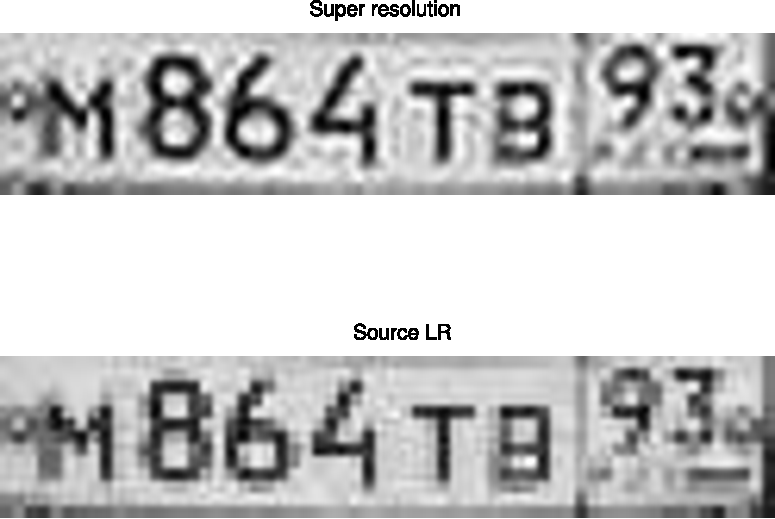
\includegraphics[width=\columnwidth]{content/compare_result_sr1.pdf}
\end{frame}

\section{SR2}
\begin{frame}{Результаты подхода}
  % This file was created by matlab2tikz v0.3.3.
% Copyright (c) 2008--2013, Nico Schlömer <nico.schloemer@gmail.com>
% All rights reserved.
% 
% The latest updates can be retrieved from
%   http://www.mathworks.com/matlabcentral/fileexchange/22022-matlab2tikz
% where you can also make suggestions and rate matlab2tikz.
% 
% 
% 
\begin{tikzpicture}

\begin{axis}[%
width=10cm,
height=7.88709677419355cm,
scale only axis,
xmin=0,
xmax=16,
xlabel={Номер изображения},
ymin=12,
ymax=35,
ylabel={PSNR dB},
legend style={draw=black,fill=white,legend cell align=left}
]
\addplot [
color=blue,
solid
]
table[row sep=crcr]{
1 27.4470571608433\\
2 22.8300247931548\\
3 22.1109193658809\\
4 22.0652635937327\\
5 23.6272496813018\\
6 21.6055079117517\\
7 21.4619565703478\\
8 26.9867634881452\\
9 20.9809477047241\\
10 23.2957078121211\\
11 23.9394056382537\\
12 25.5317267141373\\
13 29.2416356490523\\
14 24.1599986234539\\
15 23.7307351145084\\
16 22.5888532577419\\
};
\addlegendentry{Алгоритм с регуляризацией};

\addplot [
color=green!50!black,
solid
]
table[row sep=crcr]{
1 18.4503335459593\\
2 15.9429403769346\\
3 15.9459841548511\\
4 15.5934814518383\\
5 16.9838249182421\\
6 13.7171337206461\\
7 12.7696291928783\\
8 21.6627180369299\\
9 13.6838913514568\\
10 18.8295593160528\\
11 17.4771261841067\\
12 20.0919833166445\\
13 22.2356695114555\\
14 16.697098012576\\
15 18.4542205359683\\
16 15.4386868770896\\
};
\addlegendentry{Начальное приближение};

\end{axis}
\end{tikzpicture}%

\end{frame}

\begin{frame}{Пример изображений алгоритма с регуляризацией}
  % This file was created by matlab2tikz v0.3.3.
% Copyright (c) 2008--2013, Nico Schlömer <nico.schloemer@gmail.com>
% All rights reserved.
% 
% The latest updates can be retrieved from
%   http://www.mathworks.com/matlabcentral/fileexchange/22022-matlab2tikz
% where you can also make suggestions and rate matlab2tikz.
% 
% 
% 
\begin{tikzpicture}

\begin{axis}[%
width=5cm,
height=1cm,
axis on top,
scale only axis,
xmin=0.5,
xmax=50.5,
y dir=reverse,
ymin=0.5,
ymax=10.5,
hide axis,
name=plot1,
title={Начальное приближение}
]
\addplot graphics [xmin=0.5,xmax=50.5,ymin=0.5,ymax=10.5] {../plots/sr2_psnr_rising-1.png};
\end{axis}

\begin{axis}[%
width=5cm,
height=1cm,
axis on top,
scale only axis,
xmin=0.5,
xmax=50.5,
y dir=reverse,
ymin=0.5,
ymax=10.5,
hide axis,
name=plot2,
at=(plot1.below south west),
anchor=above north west,
title={Оригинальное изображение}
]
\addplot graphics [xmin=0.5,xmax=50.5,ymin=0.5,ymax=10.5] {../plots/sr2_psnr_rising-2.png};
\end{axis}

\begin{axis}[%
width=5cm,
height=3.74020102770053cm,
scale only axis,
xmin=0,
xmax=60,
xlabel={Итерация},
ymin=12,
ymax=20,
ylabel={PNSR dB},
name=plot4,
at=(plot2.right of south east),
anchor=left of south west,
title={PSNR}
]
\addplot [
color=blue,
solid,
forget plot
]
table[row sep=crcr]{
1 12.3202813060895\\
2 12.9529644677536\\
3 13.5260641864726\\
4 14.0455567679328\\
5 14.5157791626175\\
6 14.9401084698002\\
7 15.3214501720298\\
8 15.6625515600167\\
9 15.966172416695\\
10 16.2351495750173\\
11 16.4723907826822\\
12 16.6808285374995\\
13 16.8633577505267\\
14 17.022773711704\\
15 17.1617200798005\\
16 17.2826512422842\\
17 17.3878096467359\\
18 17.4792164732515\\
19 17.5586729726292\\
20 17.6277695606153\\
21 17.6878999988837\\
22 17.7402784568312\\
23 17.7859577695793\\
24 17.8258476931939\\
25 17.8607323650764\\
26 17.8912864943554\\
27 17.9180900396926\\
28 17.9416412935904\\
29 17.9623683983446\\
30 17.9806393834473\\
31 17.9967708494893\\
32 18.011035438794\\
33 18.0236682351711\\
34 18.0348722293508\\
35 18.0448229763448\\
36 18.0536725585498\\
37 18.0615529553497\\
38 18.0685789072431\\
39 18.0748503506304\\
40 18.0804544886167\\
41 18.0854675536173\\
42 18.0899563091761\\
43 18.0939793311617\\
44 18.0975881022909\\
45 18.1008279486261\\
46 18.1037388421964\\
};
\end{axis}

\begin{axis}[%
width=5cm,
height=1cm,
axis on top,
scale only axis,
xmin=0.5,
xmax=50.5,
y dir=reverse,
ymin=0.5,
ymax=10.5,
hide axis,
at=(plot4.above north west),
anchor=below south west,
title={Результат}
]
\addplot graphics [xmin=0.5,xmax=50.5,ymin=0.5,ymax=10.5] {../plots/sr2_psnr_rising-3.png};
\end{axis}
\end{tikzpicture}%
\end{frame}

\begin{frame}{Пример изображений алгоритма с регуляризацией}
  % This file was created by matlab2tikz v0.3.3.
% Copyright (c) 2008--2013, Nico Schlömer <nico.schloemer@gmail.com>
% All rights reserved.
% 
% The latest updates can be retrieved from
%   http://www.mathworks.com/matlabcentral/fileexchange/22022-matlab2tikz
% where you can also make suggestions and rate matlab2tikz.
% 
% 
% 
\begin{tikzpicture}

\begin{axis}[%
width=5cm,
height=0.9cm,
axis on top,
scale only axis,
xmin=0.5,
xmax=100.5,
y dir=reverse,
ymin=0.5,
ymax=18.5,
hide axis,
name=plot1,
title={Начальное приближение}
]
\addplot graphics [xmin=0.5,xmax=100.5,ymin=0.5,ymax=18.5] {../plots/sr2_psnr_rising_2-1.png};
\end{axis}

\begin{axis}[%
width=5cm,
height=0.9cm,
axis on top,
scale only axis,
xmin=0.5,
xmax=100.5,
y dir=reverse,
ymin=0.5,
ymax=18.5,
hide axis,
name=plot2,
at=(plot1.below south west),
anchor=above north west,
title={Оригинальное изображение}
]
\addplot graphics [xmin=0.5,xmax=100.5,ymin=0.5,ymax=18.5] {../plots/sr2_psnr_rising_2-2.png};
\end{axis}

\begin{axis}[%
width=5cm,
height=3.76301826188611cm,
scale only axis,
xmin=0,
xmax=60,
xlabel={Итерация},
ymin=16,
ymax=24,
ylabel={PNSR dB},
name=plot4,
at=(plot2.right of south east),
anchor=left of south west,
title={PSNR}
]
\addplot [
color=blue,
solid,
forget plot
]
table[row sep=crcr]{
1 16.3819645818644\\
2 17.0780369540006\\
3 17.7072119644846\\
4 18.2779056934387\\
5 18.7961056895055\\
6 19.2661449216461\\
7 19.6913393603133\\
8 20.0744644313597\\
9 20.4180785288889\\
10 20.7247161200502\\
11 20.99697867816\\
12 21.2375525901663\\
13 21.4491809002166\\
14 21.6346113256761\\
15 21.7965374526836\\
16 21.9375443813036\\
17 22.0600651225625\\
18 22.1663501942838\\
19 22.2584502336536\\
20 22.3382099167395\\
21 22.4072708002286\\
22 22.4670806035736\\
23 22.5189066898221\\
24 22.5638518996966\\
25 22.6028713265497\\
26 22.6367890211028\\
27 22.6663139523695\\
28 22.6920548161245\\
29 22.7145334789205\\
30 22.7341969841924\\
31 22.7514281393378\\
32 22.7665547601366\\
33 22.7798576811311\\
34 22.7915776553607\\
35 22.8019212700101\\
36 22.8110660003991\\
37 22.8191645163655\\
38 22.8263483445616\\
39 22.8327309788807\\
40 22.8384105200143\\
41 22.8434719145521\\
42 22.8479888543236\\
43 22.8520253879912\\
44 22.8556372892352\\
45 22.8588732191953\\
46 22.8617757150688\\
47 22.864382031827\\
48 22.8667248597992\\
};
\end{axis}

\begin{axis}[%
width=5cm,
height=0.9cm,
axis on top,
scale only axis,
xmin=0.5,
xmax=100.5,
y dir=reverse,
ymin=0.5,
ymax=18.5,
hide axis,
at=(plot4.above north west),
anchor=below south west,
title={Результат}
]
\addplot graphics [xmin=0.5,xmax=100.5,ymin=0.5,ymax=18.5] {../plots/sr2_psnr_rising_2-3.png};
\end{axis}
\end{tikzpicture}%
\end{frame}

\begin{frame}{Пример изображений алгоритма с регуляризацией}
%   \begin{tikzpicture}
%     \node (img1) {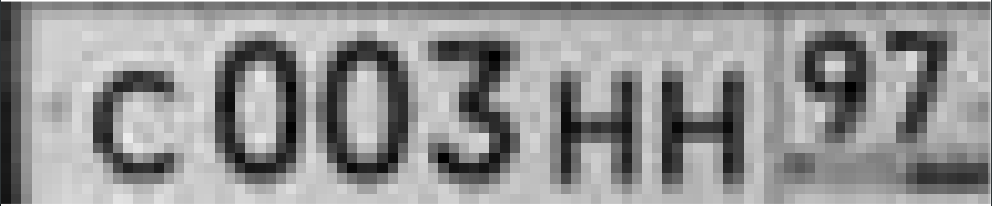
\includegraphics[width=10cm]{content/sr2_two_1.png}};
%     \node (img1) {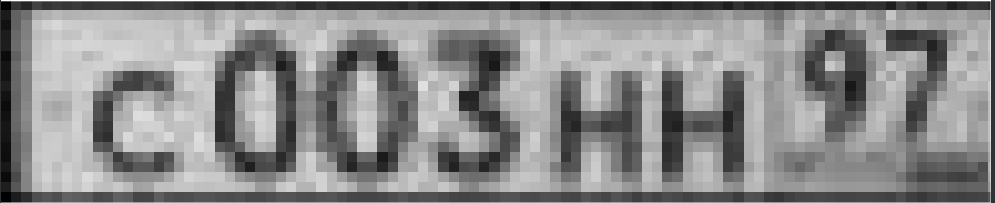
\includegraphics[width=10cm]{content/sr2_two_2.png}};
%   \end{tikzpicture}
  \begin{figure}
    \caption{Результат}
    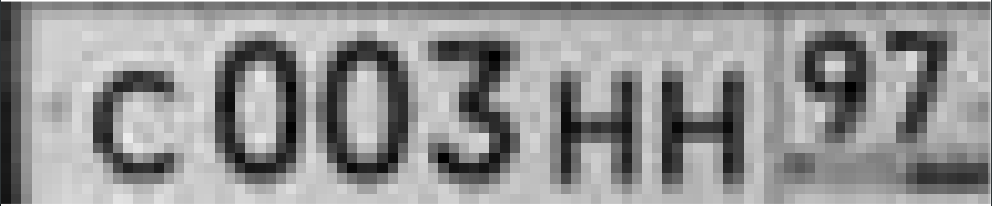
\includegraphics[width=\columnwidth]{content/sr2_two_1.png}\\
  \end{figure}
  \begin{figure}
    \caption{Начальное приближение}
    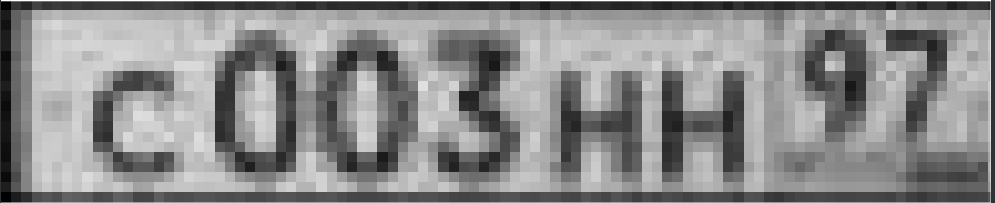
\includegraphics[width=\columnwidth]{content/sr2_two_2.png}
  \end{figure}
 %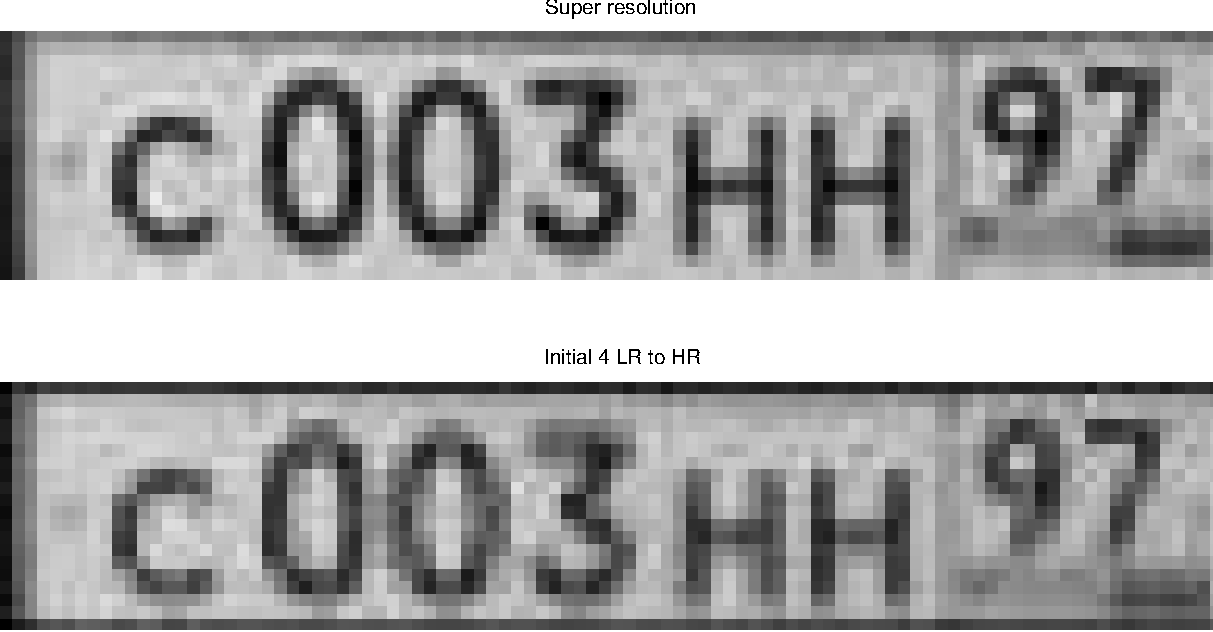
\includegraphics[width=\columnwidth]{content/sr2_two_images.pdf}
\end{frame}

\section{Результаты}

\begin{frame}{Результаты}
\subsection{Вывод} В результате опытов было установлено, что, несмотря на то, что в большинстве случаев первый алгоритм
улучшает PSNR, результаты его работы существенно хуже второго.

Второй алгоритм обладает устойчивостью к следующим шумам в исходных данных:
\begin{itemize}
  \item устойчивость к ошибкам сдвига (ошибка до 0,2 пикселя существенно не меняет результат, ошибка до 2 пикселей
    приводит к повышению PSNR по сравнению с начальным приближением)
  \item устойчивость к шуму на на исходных изображениях (нормальный шум с дисперсией $\sigma=25$ при значениях яркости
    от 0 до 255)
  \item устойчивость к размытию исходных изображений ($\sigma = 1$)
\end{itemize}
Результаты работы будут опубликованы на конференции СПИСОК-2013
\end{frame}
